\chapter{Financial background}\label{chap:HFFD}	% file "chap2.tex"

Successive improvements in the availability of high quality data have led to increasingly detailed pictures of the trade and order placement activity in financial markets around the world. Although historical datasets exist dating back to the nineteenth century, these are of low resolution: for example, the daily values of the Dow Jones Industrial Average (DJIA) at the end of each trading day.   The frequency of data collection has shifted from daily to minute, second and currently microsecond resolution -- all in the context of the multiplication of trading venues both nationally within the developed economies and internationally as new exchanges open.  The integration of such vast streams of high-frequency data into effective trading strategies has driven developments in computing infrastructure, statistical analysis, algorithm design and high-speed electronic communication. 

\section{Historical volatility}
The assessment of market volatility is important for investors, not least in providing an indication of the chance that the value of an asset will drop below an unacceptable level at some point in the future. Financial historians have devoted considerable effort to understanding the causes of volatility, focussing particularly on events surrounding dramatic falls in the stock market. Although the primary focus of this thesis is on high-frequency data, it is of interest to describe some of the historical events that have shaped modern developments in volatility research.   

\begin{table}[h]
\small
\centering
\begin{tabular}{| r | r | r | r | r |r | r | r | r |}
\hline
\multicolumn{1}{|c|}{Rank} & 
\multicolumn{1}{|c|}{Date} & 
\multicolumn{1}{|c|}{\% Chg} &
\multicolumn{1}{|c|}{Rank} & 
\multicolumn{1}{|c|}{Date} & 
\multicolumn{1}{|c|}{\% Chg} &
\multicolumn{1}{|c|}{Rank} & 
\multicolumn{1}{|c|}{Date} & 
\multicolumn{1}{|c|}{\% Chg} 
\\
\hline\hline
1	& 1987-10-19	& -22.61 & 7  & 1907-03-14  & -8.29	& 13	& 2008-10-09	& -7.33 \\
2	& 1929-10-28	& -12.82 & 8	& 1987-10-26	& -8.04	& 14	& 1917-02-01	& -7.24 \\
3	& 1929-10-29	& -11.73 & 9	& 2008-10-15	& -7.87	& 15	& 1997-10-27	& -7.18 \\
4	& 1929-11-06	& -9.92  & 10	& 1933-07-21 	& -7.84 & 16	& 1932-10-05	& -7.15 \\
5	& 1899-12-18	& -8.72  & 11	& 1937-10-18	& -7.75 & 17	& 2001-09-17 	& -7.13 \\
6	& 1932-08-12	& -8.40  & 12	& 2008-12-01	& -7.70 & 18	& 1931-09-24	& -7.07 \\
\hline
\end{tabular}
\caption{Dow Jones Industrial Average: largest daily percentage losses. Source: {\it The Wall Street Journal}. \label{table:falls}}
\end{table}

Table \ref{table:falls} shows some of the largest daily percentage losses in the past 114 years. The most notorious of these is, of course, the Wall Street crash that started on Monday, October 28, 1929. The first downward movement on Monday was followed immediately by a major drop on October 29, known as Black Tuesday.  There was then an extended period of extreme price fluctuations over months and years as the market attempted to find a new equilibrium, dropping to its lowest level on July 8, 1932. So severe was the correction that it took until 1954 for the price of the DJIA to return to the 1929 peak. See Figure \ref{fig:crashes}.

\begin{figure}[ht]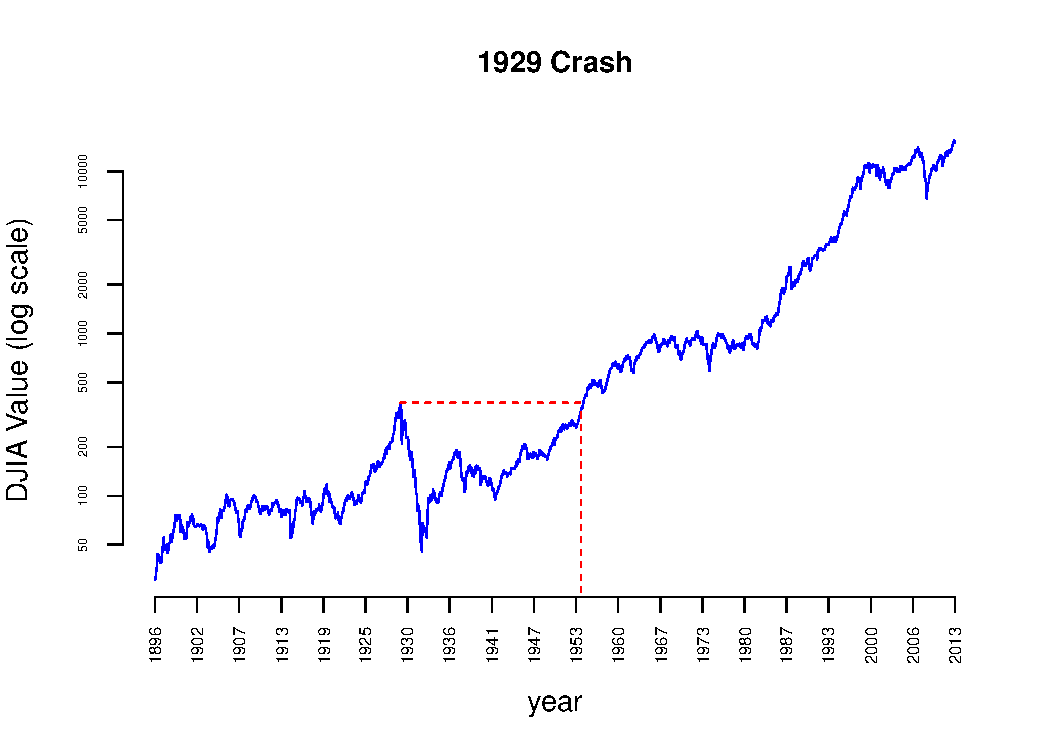
\includegraphics[width=0.5\linewidth]{./Figures/1929} 
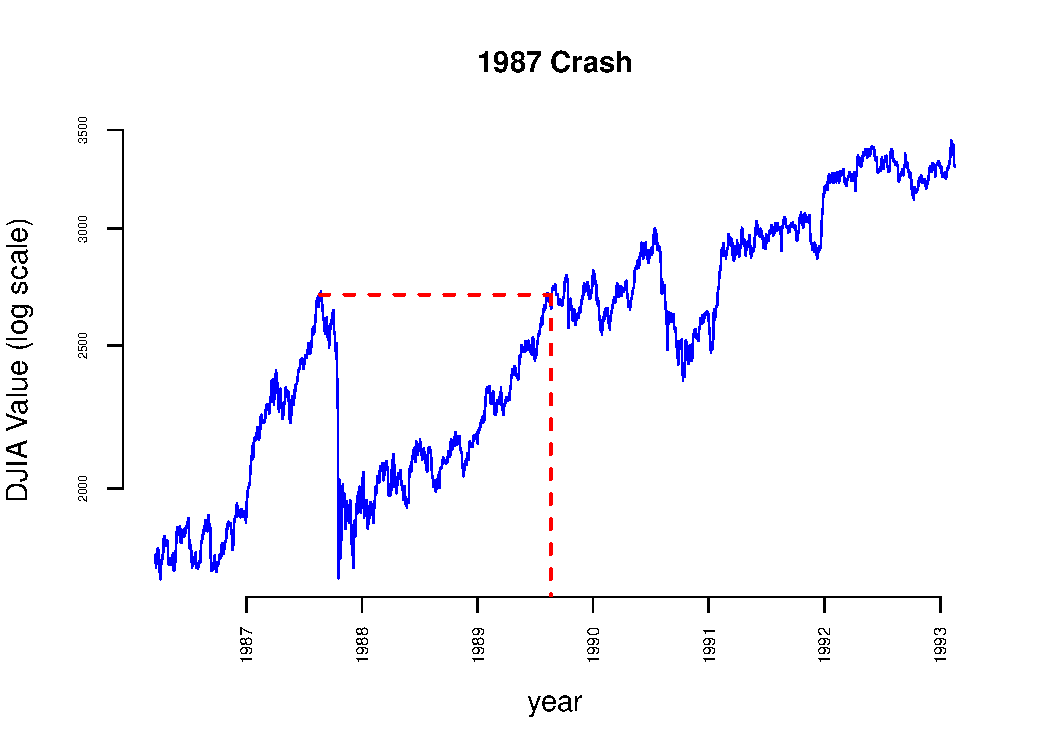
\includegraphics[width=0.5\linewidth]{./Figures/1987}
\caption{Dow Jones Industrial Average (logarithmic scale) before and after the 1929 and 1987 stock market crashes.  Recovery from the 1929 crash took almost 25 years, whereas 1987 took 2 years. Data from {\tt \small www.quandl.com}. \label{fig:crashes} }
\end{figure}

The bubble of protracted unsustainable speculation in the years preceding 1929 is generally held to be the immediate cause of the collapse \blacktext{\citep{crash1929}}.The stock market had advanced steadily for seven years and the purchase of shares with borrowed money was seen to be a guaranteed way of making money. Speculation was fuelled by a general sense of improving living standards and excitement about media and new technology such as radio. Shares in companies such the Radio Corporation of America (RCA) had reached record prices and many private investors borrowed heavily to make further investments and take advantage of the apparently one-directional price movement. When the price started to slip there was panic selling among these investors as they realised they would not be able to cover their debts. Somewhat belatedly, regulators took action to limit trading on margin in the Securities Exchange Act of 1934.    

The 1929 crash can be contrasted with the collapse of October 19, 1987, known as Black Monday.  Again there was a bubble preceding the event -- from early in 1987 until August 25, the Dow rose by 44\%. Various explanations have been advanced for the timing of the burst of sell orders that triggered the fall. For a brief account see  \blacktext{\citet{crash1987}}, and more extensively the references therein.  It is worth noting that one of the aggravating factors was the inability of the New York Stock Echange to process the large volume of trades that day and the consequential uncertainty among traders about the speed and direction in which the market was moving. Important lessons were learnt that eventually led to improved infrastructure and circuit breaking controls in the exchange. Nevertheless, despite the large fluctuation over the succeeding months in 1987, the DJIA recovered its previous value in August 1989, and  the market returned to a period of growth.  See Figure \ref{fig:crashes}.

At the turn of the century there were further collapses when the dot-com bubble burst on March 10, 2000 and when the markets opened on September  17, 2001 following the  9/11 attacks on the World Trade Centre. Both led to bursts of volatility and then eventual stability until the global financial crisis of 2007-2008 that threatened the total collapse of large financial institutions, resulting in the bailout of banks by national governments, and downturns in stock markets around the world. This too was followed by a large but temporary increase in volatility. 

In his analysis of a number of such stock market corrections, \citet{harris2002trading} observes that rapid downward movements in market valuation produce subsequent periods of high volatility.  By contrast rapid upward movements tend not to have that effect. This can be illustrated with more recent data by plotting the daily values of the S\&P 500 index and the VIX index, a implied measure of volatility derived from the Black-Scholes-Merton formula for option pricing of the S\&P 500. See Figure \ref{fig:VIX}. \blacktext{For further background on the VIX, see  \citet{investorFear}.}
The \emph{implied volatility} is the volatility obtained by using either the instantaneous or integrated version of the  option-pricing equation to match the theoretical price with the market price. It is often said to be the market's estimate of volatility. Implied volatility reflects how the market is pricing the option currently \blacktext{ \citep{impliedVol}}. Since the market does not have perfect knowledge about the future, actual and implied volatility can and will be different. In practice, implied volatility seldom matches historical volatility and this may have significant implications for hedging strategies. See for example \citet{dumas2002implied} and \citet{mykland2008infrence}.
\begin{figure}[ht]
\centering
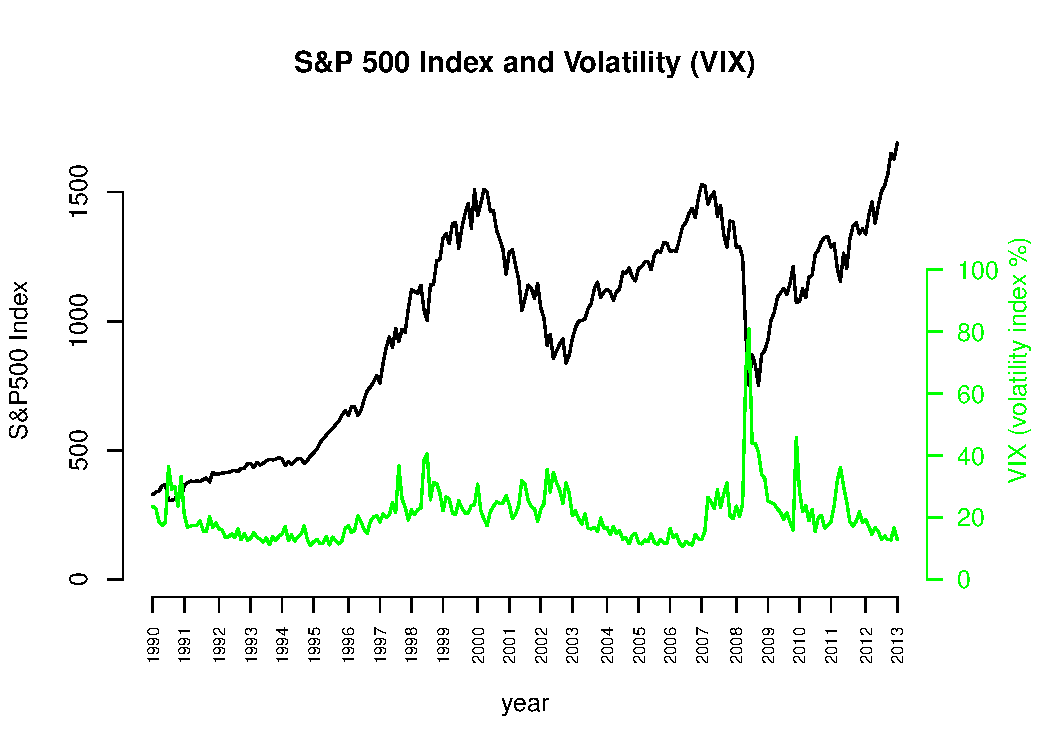
\includegraphics[width=0.95\linewidth]{./Figures/VIX} 
\caption{The volatility index (VIX) typically increases when there is a large fall in the S\&P 500 index. The highest VIX value of 80.6\% occurred on  Nov 20, 2008. Data from {\tt \small www.quandl.com}. \label{fig:VIX}}
\end{figure}

\section{Consumers of volatility research}
Volatility research is an extremely active area of research in econometrics. Building on the work of \citet{engle1982autoregressive} on ARCH models, there is an extensive well developed econometric literature devoted to the problems of volatility measurement, modelling and forecasting. The Volatility Institute at New York University Stern School of Business founded in 2009 under Engle's direction is a focus of activity providing access to advanced techniques and online volatility analyses of several thousand economic series. Similarly the Oxford Man Institute provides online access to various non-parametric measures of historical volatility updated on a daily basis.  

Econometricians are interested in establishing robust and informative summaries of price fluctuation. A wide range of such summaries have been proposed incorporating many of the well established methods of robust statistical estimation. Although the emphasis is primarily on historical analysis, the performance of these measures is often judged in a model framework, with specific models of stochastic volatility and covolatility. Descriptive measures are then scored and assessed with regard to their ability to estimate properties of the theoretical model. \blacktext{For a comprehensive review on forecasting volatility in financial markets, see \citet{forecastVol}.}

The perspective of investment managers is somewhat different. Here the main focus is on prediction of the scale of future price fluctuation and the implication for risk assessment \blacktext{\citep{assetAllocation}}. At a simple level, it may be of interest to predict the variance of the price of some asset at some future point in time. Similarly when a portfolio of assets is held, the correlation between assets become important since these will determine the optimal allocation of assets so as to minimise variability in the combined value of the set of assets. Since volatility and covolatility are known to be persistent in financial time series, model based predictions of volatility are clearly of interest and form an essential part of any investment strategy.  These models are then tested and validated with historical data. Directional price movement on the other hand cannot persist for extended periods, since that would offer obvious \emph{arbitrage} opportunities. This topic is developed in Chapters \ref{chap:volatility} and \ref{chap:covolatility}.

For both econometricians and investment managers, minor fluctuations on very short time scales are not of great importance and are treated as noise. However high-frequency traders focus on these and make their living by identifying and taking advantage of short lived opportunistic price fluctuations. They are sometimes referred to as \emph{noise traders}. Their time scale is in fractions of seconds. Mid-frequency traders have perspectives of a few minutes.  

Although there is already a considerable body of research in this area, the need to predict volatility and quantify its effect on a wide range of time scales continues to be of importance. Modern approaches are outlined in Chapters \ref{chap:volatility} and \ref{chap:covolatility}.

\section{The trading environment}
To exploit opportunities presented by price movements in financial markets traders  need access to liquidity. In financial terminology, {\it liquidity} describes the ability to trade {\it large quantities} of an asset {\it rapidly} and at {\it low cost}. Exchanges and other trading venues serve to provide liquidity by facilitating contact between buyers and sellers, either transparently by exposing buying and selling interest at specific prices and specific quantities in the case of traditional exchanges, the so-called ``lit'' venues, or in a guarded sense in the relatively unregulated world of dark pools where trades are executed on a private discretionary basis without publicly revealing the level of buy and sell interest. 

The unlit venues emerged in the the early 2000s partly as a response to the concerns of traditional traders about the impact of computer driven algorithmic trading on the working of established exchanges \blacktext{\citep{BankingMarkets}.} Nevertheless, traditional exchanges continue to provide significant sources of liquidity and active participants continue to play traditional roles. Market makers post offers to buy and sell relatively small lots but adapt rapidly to demand. They are small scale liquidity providers, making money from the difference between their buy and sell prices and also from commission paid by equity exchanges on successful execution. Opportunistic fast traders look for small pricing anomalies and trade accordingly -- they remove small scale liquidity. Block traders handle large orders for specific clients. Their role is to split these blocks into smaller lots and execute the trades without significant market impact. Other traders analyse the fundamental value of the asset and trade when they believe it is mispriced. They provide {\it resiliency}. In principle their trades ultimately result in prices reverting to those that represent the fundamental value. For further background, see 
\blacktext{\citet{microstructure}}.

\subsection{Latency}
Speed has always been important in trading environments \blacktext{ \citep{lowLatency}}. Rapid information flow between national and international financial centres will determine trading decisions.  Market data derived from different sources will have varying delays in arrival.  Even the very best sources (perhaps co-located with the exchange) will have a delay (latency) measured in milliseconds (or possibly microseconds) between the event occurring and notification being received by the relevant system. Data transmission times become very important when the system is physically some distance from the data source.  To minimise latency, high-frequency trading companies invest substantial sums in building fast communication networks between their installations. For example, if a trading event occurs on an exchange is in New York, latencies of around 30 milliseconds can be achieved for the data to be received in London via a transatlantic fibre-optic cable.  

In general, it is desirable to know, to the nearest microsecond, the original time of a trading event.  There are two reasons for this:  to provide an accurate time series for the calculation of volatilities and correlations, and to determine the effective latency as it varies under specific market conditions.  For this latter to be useful, the timestamps of the source must be related to a GPS time source, as must those of the receiving system  \blacktext{ \citep{utcTime}.} Many modern exchanges provide this type of timestamp.  However, some do not, particularly for trade data, to prevent high-frequency algorithms taking too much advantage of the pattern of activity.  Aggregated sources such as Reuters Selectfeed often do not provide this type of information.

Some Electronic Communication Networks (ECNs) such as EBS provide data on a sampled basis, rather than immediately as prices change.  The ECN may send updated information at 100ms intervals for example, posting the price range of trades in the previous 100ms time slice and a snapshot of the order book.  This may therefore hide details of multiple trades and other price movements in that period \blacktext{\citep{highFreqFX}.}

In Chapter \ref{chap:lagCorrelation} we show how to use cross-asset measures of correlation to estimate transmission delays and quantify lead-lag response times. We show for example that the recent use by high-frequency traders of proprietary microwave links on the New York to Chicago route has reduced data transmission times to around 4.5 milliseconds, close to the light-speed determined minimum of 4 milliseconds.


\section{Financial datasets: terminology}
Detailed financial data on a second-by-second basis started to be available in the 1980s.  The foreign exchange market was structured as an electronic/telephone market at that time. Currencies were priced against the US dollar.  The prices that banks and other major players were prepared to buy and sell various currencies were posted publically and updated on the pages of news services such as Reuters and Telerate. These prices would fluctuate competitively throughout the day -- the so-called {\em fighting-screen} -- partly with a view to keeping the names of the players visible as often as possible.  \blacktext{For a review of the evolution of the foreign exchange market see \citet{king2011foreign}.}

At any particular moment in time, a market trader could telephone any of these players to negotiate a price to buy or sell a specified amount of the currency. But there was no commitment to the price previously advertised on the news service. In the 1980s, data on this succession of posted prices were made available for statistical analysis, although the actual trades were private. The data consisted of a price to buy and sell a particular currency with a timestamp identifying when the price were offered. The timestamps were irregularly spaced -- updating very rapidly during periods of financial uncertainty.  These data formed the basis for early statistical analysis by \citet{zhou1996high} where it was assumed that the posted prices reflected a theoretically correct value, the efficient price, but with an added noise term recognising uncertainty.  This model (coinciding with a similar model proposed by \citet{roll1984simple} in another context) became the standard assumption in the statistical analysis of market data, giving rise to an extensive literature. See Chapter \ref{chap:volatility}. 

In the intervening years, markets have become progressively more open. Many financial assets, including foreign exchange, are now traded on ECNs and exchanges, where firm prices and quantities are quoted continuously and trades are reported with prices and amounts.           

\subsection{Exchange based trading}

The {\it limit orderbook} is the basic framework within which modern high-frequency data are monitored and processed \citep{harris2002trading,dacorogna2001introduction,hasbrouck2007empirical}.  Price data for exchange-traded instruments fall broadly 
into two categories:  quotes and trades done. In an orderbook-driven market, offers to buy and sell (\emph{quotes}) are made by market-makers, and taken by institutions wishing to trade.

In statistical terms, the limit orderbook is essentially the realisation of a tightly coupled multivariate marked point process. Observational data for a given financial asset are provided by an exchange on which it is traded. The orderbook shows how many units of the asset are available for sale by market participants at various prices per unit. These are called \emph{ask} or \emph{offer quotes}. At time $t$ we denote the cheapest ask price by $P_t(a_1)$ and the total quantity available at that price by $Q_t(a_1)$.  There will also be amounts quoted at other (worse) prices. We denote these successively worse prices by $P_t(a_k)$ with associated available quantities $Q_t(a_k)$ for $k=2,3,\dots$. 

On the other side, there are market participants who want to buy the asset. They are said to be \emph{bidding to buy} at various \emph{bid prices}. At time $t$ the highest bid price is denoted by $P_t(b_1)$, possibly quoted by several participants, and the combined quantity looking to be bought at that price is denoted by $Q_t(b_1)$. Of course, at the same time there will be others wishing to buy at cheaper prices. We denote these successively lower prices by $P_t(b_k)$ and the associated quantities by $Q_t(b_k)$, $k=2,3,\dots$.  For a particular  exchange, only $m$ values of the bid/ask quotes are published and viewable by subscribers to the data feed. The number of rungs in this ladder of quotes is typically $m=3,5$ and $10$. All the while quotes remain on the orderbook we refer to them as \emph{resting orders}. 

At time $t$ the published prices are always ordered by 
\begin{equation}\label{eq:levels}
 P_t(b_m) < \dots < P_t(b_1) < P_t(a_1)< \dots <P_t(a_m).
\end{equation}
The process $P_t(a_1) - P_t(b_1), t >0$ is called the \emph{spread}. Prices are discrete valued and for heavily traded assets usually recorded to at least 4 places of decimals. The minimum price movement is called the \emph{tick size} or \emph{pip}. The term `tick' is derived from the tick of a ticker tape and the term \emph{tick-by-tick data} denotes the sequence of data delivered  by such a device, or its modern electronic equivalent. For heavily traded assets, the spread is almost always equal to the tick size. The data associated with an orderbook are said to be high-frequency if there is a large number of changes in a brief period of time. For example, there are usually more than  3 million changes per day in the 5-level orderbook for futures trading of the S\&P index. These include changes in prices, changes in amounts available at specific prices and records of completed trades. The interval between changes may be as small as a few microseconds.

During the day the orderbook changes from time to time as new orders arrive or existing ones are cancelled.  The point processes associated with these changes are $\{N_t(a_k), t>0\}$ on the ask side and $\{N_t(b_k), t>0\}$ on the bid side, $k=1,\dots,m$, with associated marks corresponding to changes in the available quantities.  

The orderbook is also affected by trading, in one of two ways. The first is when a matching quote arrives. For example a bid quote may arrive at a price that is matched by an ask price. When the amount in the arriving quote is matched completely, the ask price is consequently removed. Any unmatched units in the quote than become a bid quote for the residue.  If on the other hand, only part of the order is matched (because of insufficient available quantity) the ask price is unchanged but the amount at that ask price is adjusted accordingly. 

Alternatively, trades can be submitted to the exchange on an \emph{immediate or cancel} (ioc) basis, meaning that if for example the trader sends an order to buy $n$ units of the published amount offered at the best ask price, then the deal is done for the minimum of $n$ units and the amount still available at the time the order arrives at the exchange. The ioc order is cancelled by the exchange if there are no units available at the target price (either because another trader has got there first or because the offered price has been withdrawn).  

In both cases we can distinguish between trades that were completed at the existing ask price and those that were completed at the bid price. We denote the sequence of trade times by $\mathcal{T}^*(a)$ and $\mathcal{T}^*(b)$, respectively, with marks given by the associated price and size of the trade. Trade data (timestamp and price) are generally published by the exchange. The size of individual trades may not be given, although it can be inferred to some degree of accuracy from changes in the order book.  
\begin{figure}[ht]
\centering
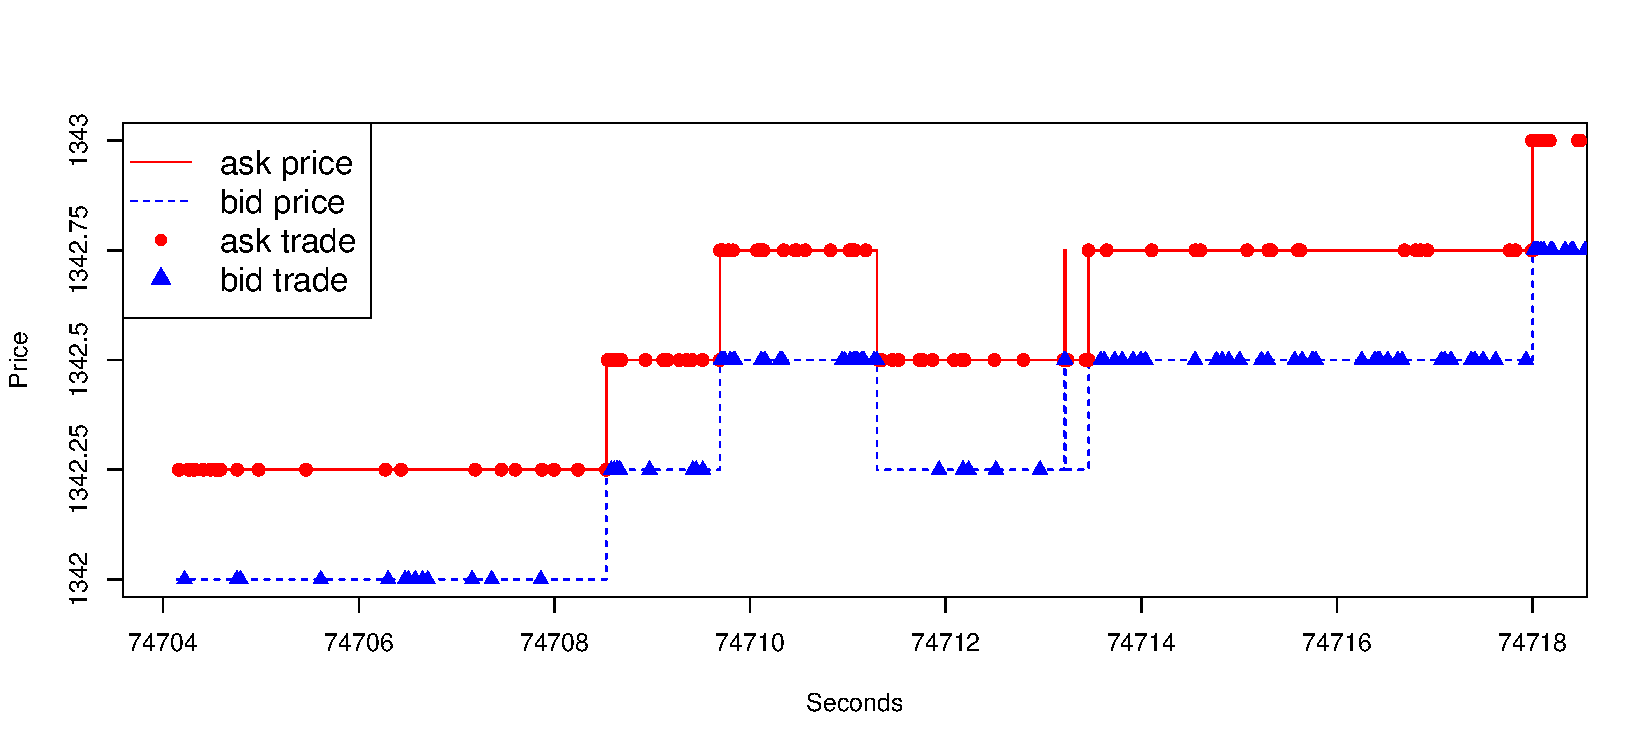
\includegraphics[width=\linewidth]{./Figures/OBLevel1}
\caption{Prices and trades at the first level of a limit order book \label{fig:OBLevel1}. }
\end{figure}
Figure \ref{fig:OBLevel1} is a small snapshot of the first level of the S\&P 500 index futures limit orderbook. The picture is typical, showing large numbers of trades in between relatively slowly changing prices. 

This pattern is a comparatively recent development in orderbook trading. Twenty years ago trades were less frequent and individually much larger. The dominance of algorithmic trading in recent years has led to computer controlled strategies for the rapid submission of many small orders, in part with the aim of disguising the intention to buy and sell larger amounts of the asset  \blacktext{\citep{hasbrouck2009technology}.}

For some purposes, the simple sequence of trade times $\mathcal{T^*}$ and associated prices $P$, without distinguishing between bid and ask, is taken to be a basic summary of market activity. For some assets, $(\mathcal{T^*},P)$ may be the only data available. 

\begin{figure}[ht]
\centering
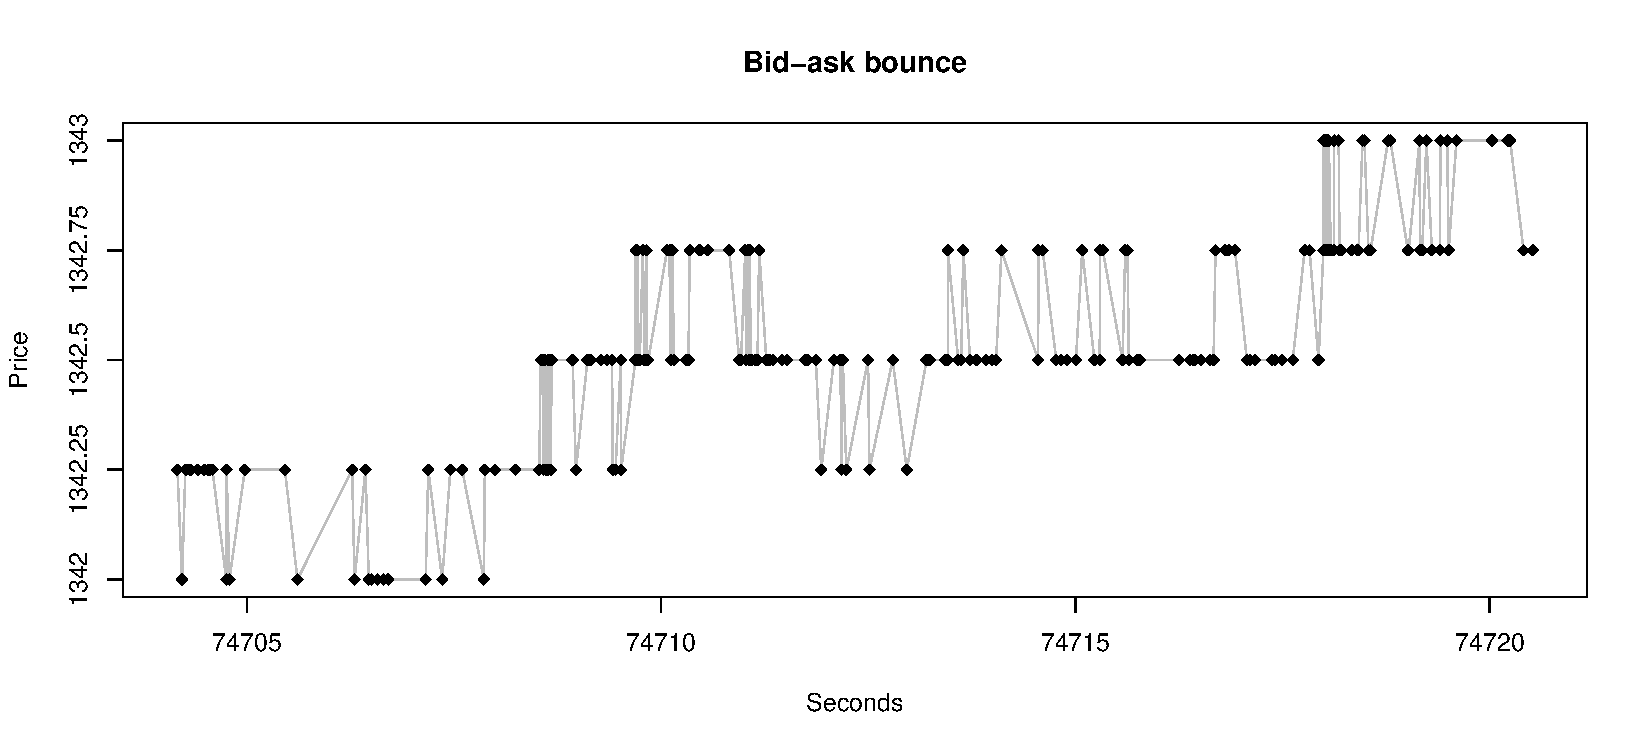
\includegraphics[width=\linewidth]{./Figures/OBbounce}
\caption{Trade price from a limit order book over a 15 second interval -- illustrating bid/ask bounce \label{fig:OBbounce}. }
\end{figure}

Note that trade prices on either side of the book (bid and ask) will necessarily be separated by the spread.  This explains the small rapid changes in trade prices seen in the simple sequence $S$, illustrated in Figure \ref{fig:OBbounce} -- a phenomenon known as \emph{bid/ask bounce}. It is one aspect of what is known as \emph{microstructure noise}.  

On a longer time scale, these changes are negligible and trade prices can move widely as in Figure \ref{fig:OBbib1hours}.
\begin{figure}[ht]
\centering
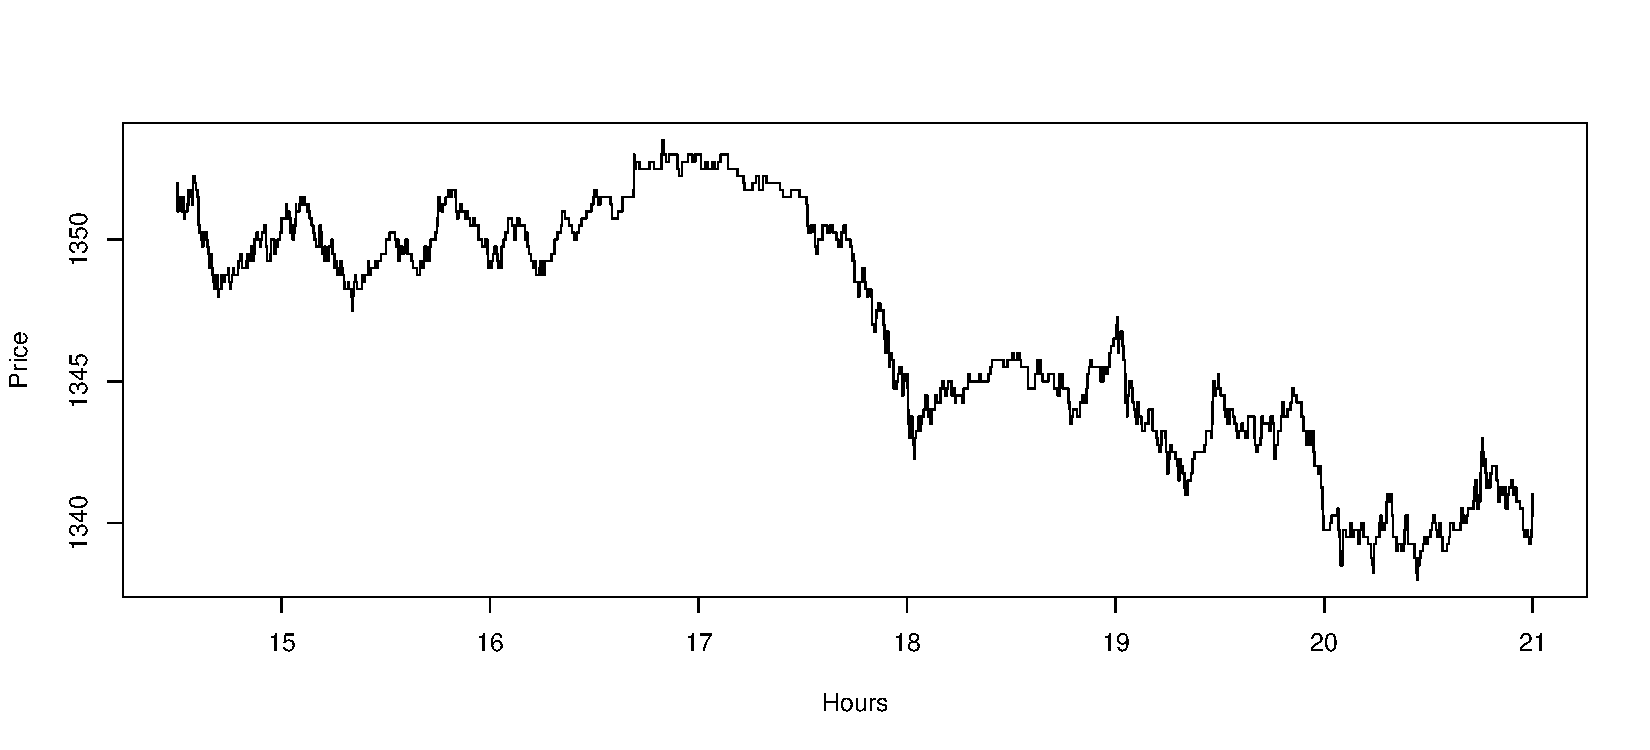
\includegraphics[width=\linewidth]{./Figures/OBbib1hours}
\caption{Trade price data over the course of the trading day (CME S\&P 500 index futures) \label{fig:OBbib1hours}. }
\end{figure} 

\subsection{Choice of observables}\label{sec:observables}
When working with orderbook data, there are a number of options in deciding which variables to use and when to observe them \blacktext{ \citep{engle2002analysis}.} Nowadays exchanges provide detailed price information in a more or less continuous stream. The first option is not to subsample at all, i.e.\ use all the data --  but this may present substantial computational costs when considering a time sequence that ticks whenever there is any change in the orderbook at all. Another option is to time slice at regular intervals: per second, per minute, etc, but this risks missing important localised activity within particular time slices. Other options are slicing at trade times or changes of the best bid and ask prices  $P_t(b_1)$ and $P_t(a_1)$ and there are further options of working with a time scale on which volatility is approximately constant. We return to this topic at several points in later Chapters. For further background see \citet{pigorsch2012volatility}.

The mid-price $m(t)$ is a useful summary of an order book. In the simplest form it is the unweighted average of the best bid and ask prices at each time $t$, i.e.\
$$ m(t) = \frac{P_t(a_1) + P_t(b_1)}{2}.$$
A weighted version $w_t$ is often used too, taking account of the amounts available at the best price, $Q_t(a_1)$ and  $Q_t(b_1)$, inversely weighting so that
$$ w_t = \frac{P_t(a_1)Q_t(b_1) + P_t(b_1)Q_t(a_1)}{Q_t(a_1) + Q_t(a_1)}.$$
More elaborate measures of the central price on the orderbook take account of further rungs in the orderbook ladder.  
 
Figure \ref{fig:OBLevel5} shows some tick-by-tick data in greater detail. These are  data that ``tick'' whenever a trade is reported or the quoted amount changes at any of the 5 levels on either side of the order book. For S\&P 500 index futures there may be around 3 million ticks per day. Each tick is time stamped by the exchange to microsecond accuracy.
\begin{figure}[ht]
\centering
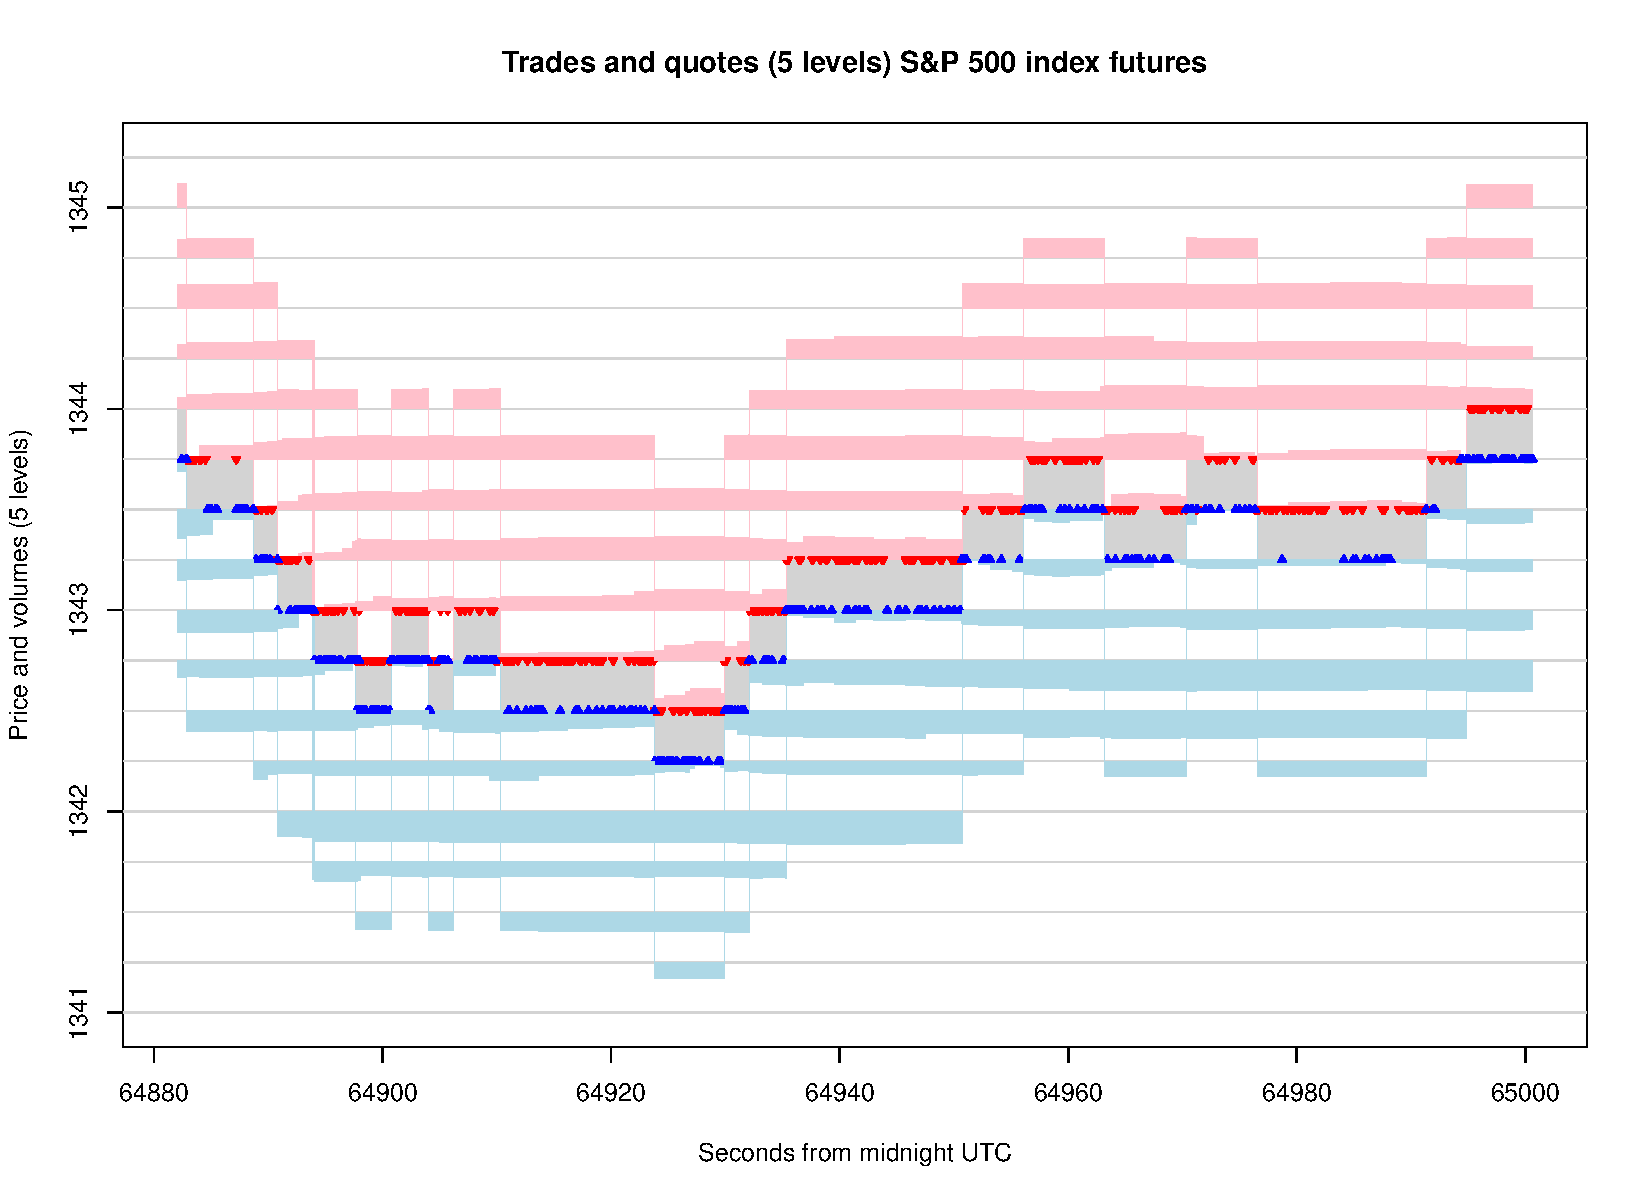
\includegraphics[width=\linewidth]{./Figures/OBLevel5} 
\caption{Example of order book and trades data, tick-by-tick, for S\&P 500 index futures: 120 second interval, around 25000 ticks, 5 levels. The volumes quoted at each price are illustrated by coloured shading. The spread region is shaded grey. Trades are marked by triangular symbols. Trade sizes range between 1 and 5000 contracts. \label{fig:OBLevel5} }
\end{figure}

In principle, volatility estimates can be obtained for any such sequence of exchange data.  In one sense trade data is a more solid reflection of market activity since it reflects active decisions, but high-frequency trading requires knowledge of the {\it immediate future} volatility and for this purpose the quoted prices and the general structure of the order book may be more informative.

\section{Sources of high-frequency data}
High-frequency computerised trading systems are geared towards markets with substantial trading activity. 
Traders tends to gravitate towards markets that are highly liquid.  Liquid markets are characterised by an ability to absorb trading activity without substantial price movement. In other words, there are substantial volumes available to buy and sell and these amounts are rapidly renewed by a broadly based cohort of market participants whenever trades take place. High-frequency market-making firms play an important role in the provision of liquidity, thereby ensuring that prices are stabilised with the minimum difference between buying and selling prices. 

Equity dealing on the major electronic exchanges around the world is an important focus as is foreign exchange trading. Alongside these cash markets, a wide variety of futures contracts are available and traded heavily on futures exchanges such as the Chicago Mercantile Exchange, Eurex in Frankfurt and Atlanta-based Intercontinental Exchange (ICE).

\subsection{Futures}         
Futures are contracts to buy or deliver a certain quantity of a specific asset at a fixed point of time in the future, the expiry time of the contract \citep{hull2009options}. The buyer of such a contract is said to be {\it long} and the party who promises to deliver is said to be {\it short}. In their original form, futures were contracts to deliver physical quantities such as foodstuffs at a specified price. Gradually in recent years, exchanges have extended the idea to less tangible assets where delivery is either impossible or rare.  For these cases, delivery is eventually settled by cash equivalence with daily margin calls on the holders of the contract to reflect the inherent risk and value of the contractual obligation. \blacktext{ For further details see \citet{miller1986financial}.}

\subsection{Eurodollar and other interest rate futures}
It may be helpful to illustrate the mechanics of Eurodollar futures trading. The 3-month London Interbank Offered Rate (LIBOR) is a pooled estimate of the cost of borrowing US dollars in the financial markets outside the United States for a 3-month period. Eurodollar futures contracts depend on the future value of LIBOR at specified expiry dates \citep*{CMEEurodollar}. The contracts are traded heavily on the Chicago Mercantile Exchange (CME). Clearly there is no tangible asset here, although the current 3-month LIBOR is published daily and will eventually be known at the specified expiry date of the contract. Meanwhile an assessment of the rate can be made. 

By convention the contract trades with a `price' that is  100 minus the annualised interest rate.  So if there is a consensus that the annualised 3-month LIBOR will be 1.01\% at the expiry date of the contract, the notional `price' will be approximately 100 minus the rate, i.e.\ 98.99. Some traders will assess the price higher and some lower. 

The Eurodollar futures contract is based on lending a notional \$1 million. A trader who is short the contract agrees to deliver a synthetic product created at the expiry date with a value of $ \$1 \text{ million} \times (100 - x)$, where $x$ is the annualised 3-month LIBOR on that date.  Similarly, a trader who is long agrees to buy the product at this value.

As the expiry approaches, the exchange transfers money between the traders with short and long positions, adjusting for their respective anticipated financial commitments at expiry. A movement of one basis point, one hundredth of a percentage point, equates to a value of \$25, by the calculation
$$ \$25 = (\$1 \text{ million}) \times (0.01 \text{ percent per year}) \times (90 \text{ days}/ 360 \text{ days per year}).$$  Money is transferred between those with short and long positions on this basis.
In fact, the number of days in a 3 month period is not exactly 90, and the notional \$1 million is re-interpreted by the exchange and varied from quarter to quarter, to preserve the simple value of \$25 per basis point movement.         

For Eurodollar, there are individual contracts for each of the quarterly expiry months: March, June, September and December for 10 years into the future along with 4 monthly expiry dates for the nearest months not in the quarterly cycle. In addition there are spread contracts where the trader takes a long position in the contract for one expiry date and a short position in a subsequent expiry, a {\it calendar spread} and more complicated combinations involving contracts with 3 or more expiry dates. The contracts are highly correlated with strong linear relationships  {\blacktext{  \citep{jegadeesh1996behavior}.}             

\subsection{Government bond futures}
Government bond futures operate in a similar manner to interest rate futures such as Eurodollar.  The most frequently traded are US Treasury and German bond futures. Contracts are defined by the exchange which is used to trade them, and specify various parameters of the trade being done, including the quantity of the underlying instrument (e.g.\ \$100,000 bond) and the delivery date, which is usually set to be one of 4 specific times each year (March, June, October, December). Again futures trading does not necessarily result in delivery of the underlying instrument - a contract may be bought and subsequently sold to result in no outstanding position (liability to deliver or receive). 
Since futures contracts are specific to a single exchange, they are identified by a code defined by the exchange.  For example, 10-year US treasury futures contracts on the CBOT Globex electronic exchange are identified by the code ZN.  The specific maturity date is then appended as a further two character code - for example, ZNZ9 refers to the contract for delivery in December 2009. \blacktext{For further details see \citet{burghardt1994treasury}.}
\subsection{Other futures contracts}
Equity Index futures contracts are based on the projected values of equity indices such as the S\&P 500 index of share prices on the New York Stock Exchange, the FTSE index in London and the equivalent indices on the Frankfurt exchange. 
Foreign Exchange (FX) futures contract follows the exchange rates between major currencies.  The CME exchange is the most active market for FX futures. 
\subsection{Cash FX}  
Cash FX data relate to the current spot rate between two currencies.  So for example, GBPUSD spot refers to the number of US dollars that one pound sterling will buy for spot delivery (2 days from today). In our context the trading ECNs include Reuters and Electronic Broking Services (EBS) that is an electronic inter-dealer broker and provider of post-trade services. 

The FX orderbook as with other limit orderbooks contains a `ladder' of prices, with the bid-offer price spreads varying according to the quantity on offer.  For example, 1 million USDJPY might be offered at 90.48/90.50 whereas 20 million could be offered at 90.47/90.51. The top `rung' of the orderbook - i.e.\ that with the narrowest and therefore best spreads - is quoted as the best bid/ask data and generally available via electronic quoting services such as Reuters IDN Selectfeed.  In the case of FX this may be a blended, or `best' rate spanning multiple exchanges.  

An example of high-frequency FX data from EBS is given in Table \ref{FXtable}.

\begin{table}
\begin{center}
\begin{minipage}{0.9\linewidth}
{\scriptsize \begin{verbatim}

time        reg_b1  reg_a1  b1     qb1    a1     qa1      given     paid
53731.41 	  90.12	  90.21   90.17	   4    90.18	   5          0        0
53731.513	  90.12	  90.21   90.17	   4    90.18	   6          0        0
53731.61 	  90.12	  90.21   90.17	   3    90.18	   6      90.17        0
53731.711	  90.09	  90.2 	  90.15   15    90.16	  10      90.16        0
53731.811	  90.1 	  90.2 	  90.15	  11    90.16	   4          0    90.16
53731.91 	  90.09	  90.2 	  90.15	   5    90.16	   3          0    90.16
53732.017	  90.09	  90.2 	  90.15	   5    90.17	   9          0        0
53732.109	  90.09	  90.2 	  90.15	   5    90.16	   1          0        0
53732.208	  90.09	  90.2 	  90.15	   4    90.16	   1          0        0
53732.309	  90.09	  90.2 	  90.15	   3    90.16	   1          0        0
53732.415	  90.08	  90.2 	  90.15	   2    90.16	   1          0        0
53732.708	  90.08	  90.2 	  90.15	   2    90.16	   1          0        0
53733.306	  90.08	  90.2 	  90.15	   2    90.16	   1          0        0


time      - time, in seconds of day

reg_b1    - regular bid (i.e. price you can sell a regular amount)
reg_a1    - regular offer (i.e. price you can buy a regular amount) 
qb1       - volume at bid on the top of the book (i.e. volume at b1)
qa1       - volume at offer on the top of the book (i.e. volume at a1)
b1        - bid at the top of the mkt orderbook
a1        - ask at the top of the mkt orderbook

given     - last price given (sold)
paid      - last price paid (bought)

\end{verbatim}}
\end{minipage}
\end{center}
\caption{Example of foreign exchange data from EBS \label{FXtable}}
\end{table}

Note that, these EBS records are time-sliced at approximately 100 millisecond intervals. The quote data, price and volume, are correct at each time interval but the trade data only provide the best price of a trade in the time interval and do not show how many trades occurred or the corresponding trade volumes  \blacktext{\citep{chaboud2014rise}.} On the EBS system in operation when these data were collected, FX prices could only change by multiples of 1\% of a basic unit which is a 1/100 dollar for the US currency. The terms `regular bid' and `regular offer' above refer to the price the trader would have to pay to sell or buy a fixed amount of the currency, e.g.\ 50 million US dollars when exchanging Japanese Yen. For EBS, traders are additionally able to view the volume of currency available at certain prices above and below the bid and ask prices. Underlying all of this is a complicated automated process managed by the ECN, dealing with high-frequency submissions and deletions of quotes -- but that is hidden from the trader.   

The difference between the data formats of FX and bond futures presents a difficulty in estimating cross-correlations before between these two assets. This is discussed further in Chapter \ref{chap:covolatility}.

